\chapter{Machine Learning Quantum Materials}

Session 9 closed by turning linear response into a diagnostic tool and running it across
essentially every system class the course had built: metals, superconductors, topological matter,
quantum magnets. That session was a synthesis session in a narrow sense, one formalism applied
everywhere. Today's session is a synthesis in a much broader sense: we are going to step back from
condensed matter for a moment and ask what happens when we let machine learning talk to everything
we have built over the last nine sessions, in both directions. Sometimes machine-learning
architectures will turn out to be exactly the right tool for a hard many-body problem; sometimes,
rather wonderfully, the reverse will be true, and a many-body technique we already know will turn
out to be exactly the right architecture for a machine-learning problem. This is also, quite
deliberately, the last session of the course, and before we start we should be upfront about one
practical difference from every session before it: \textbf{there is no companion Jupyter notebook for
this topic}. The \texttt{jupyter-notebooks/} folder stops at \texttt{session9.ipynb}, so today's notes carry no
``try it in the notebook'' callouts anywhere, not because the material is any less hands-on in
spirit, but because that particular piece of infrastructure was not built for this session. Treat
today's derivations as the thing to sit with directly on the page.

The session closes the course's arc in two deliberate ways, and it is worth naming both before we
start. First, we are going to build neural network quantum states from the ground up. This is the
first time the course meets the idea in full: a neural network standing in for the exponentially
many coefficients of a many-body wavefunction, trained by turning the variational principle itself
into a loss function, occupying its own place in the hierarchy of variational many-body states
alongside matrix product states and projected entangled pair states, and reused a second time for
reconstructing wavefunctions from a handful of measurements. Second, and this is the genuine
full-circle moment, we are going to meet Hamiltonian learning, which is the literal inverse of the
very first move this course ever made. Session 1 opened by saying: give us a Hamiltonian, and we
integrate the Schr\"odinger equation forward to get observables. Today's closing topic starts from
observables and asks for the Hamiltonian. Ten sessions after we first wrote that forward arrow
down, we get to reverse it.

\section{Two directions of traffic between machine learning and many-body physics}

Let us set the map for today, because the session genuinely runs in two directions and it helps to
know which way we are facing at each point. In one direction, we use machine-learning
architectures, mostly neural networks, to attack many-body problems: representing wavefunctions
too large to store, reconstructing states from a handful of measurements, classifying phases of
matter, learning Hamiltonians from experimental observables. In the other direction, we use
many-body architectures, tensor networks in particular, as machine-learning tools in their own
right, applied to ordinary tasks like image classification. And running underneath both directions
is a third theme, arguably the most practically important one: combining machine learning with the
condensed-matter machinery we already have (density functional theory, phase classification,
Hamiltonian extraction) to attack problems that are hard for either approach alone. The order we
will follow, matching how the lecture actually unfolded, is: neural networks and how they learn,
neural network quantum states and tomography, tensor networks repurposed as machine learning,
machine learning inside density functional theory, phase classification, and finally Hamiltonian
learning.

\section{Neural networks as function approximators}

Machine learning is a large field, and it is worth being precise about which corner of it we are
using today. Three broad task types are worth naming. \textbf{Supervised learning} maps labeled inputs
to outputs, image classification being the standard example, and it is the one we will build on for
the rest of the session. \textbf{Generative learning} models a probability distribution directly, so
that one can \emph{sample} new instances of it; a generative adversarial network trained on photographs
of cats, for instance, can produce photorealistic images of cats that never existed. \textbf{Reinforcement
learning} trains an agent to choose actions that maximize a cumulative reward, given the state of
its environment. We will not develop generative or reinforcement learning further today (though
both have real uses elsewhere in quantum materials); the GAN cat-face example is worth keeping in
mind purely as a reminder that supervised learning is not the whole of the field, even though it is
the whole of today's toolkit.

A deep neural network is best thought of as a very flexible, parametric function. It takes an
input (an array of numbers), passes it through a sequence of layers, and produces an output (another
array of numbers). Within a layer, each node's value is a nonlinear function of the values of all
nodes in the previous layer, combined with a set of free parameters: the \emph{weights} (one per
connection) and \emph{biases} (one per node). The architecture, the number and width of the layers, sets
how complex a function the network \emph{can} represent; the specific values of the weights and biases,
collectively $\theta$, set which function it \emph{does} represent at any given moment. Training a
network means searching over $\theta$ for the values that make the network implement the function
we actually want. Concretely, we define a \textbf{loss function} $\mathcal{L}(\theta)$ that measures how
far the network's output is from the desired one, and we minimize it, typically using
backpropagation (an efficient, exact way of computing $\partial \mathcal{L}/\partial\theta$ via the
chain rule) combined with gradient descent:

\begin{equation}
\mathcal{L}(\theta) = \sum_n \left\| f_\theta(x_n) - y_n \right\|^2, \qquad \theta \;\longrightarrow\; \theta - \eta\, \nabla_\theta \mathcal{L}(\theta),
\end{equation}

where $\{(x_n, y_n)\}$ is a set of labeled training examples and $\eta$ is the learning rate. Every
use of a neural network in this session, however exotic the physics attached to it, is a variation
on (10.1): identify the right input, the right output, and the right loss, and the training
procedure is always the same gradient-descent machinery.

The concrete example to keep in mind, because we will reuse its exact architecture twice more
today, is cat-versus-dog image classification. An image is an $N\times N$ matrix of pixel values;
we flatten it into the network's input layer, and the output layer has just two nodes, with the
target $(1,0)$ for ``cat'' and $(0,1)$ for ``dog.'' We train on a labeled set of images, minimizing
(10.1) with $f_\theta$ the network's output and $y_n$ the one-hot label, and once trained, the
network classifies new, unlabeled images. This is a genuinely reusable template: nothing about it
depends on the input being a photograph, only on it being an array of numbers with a categorical
label attached. We will meet the very same input-matrix-to-one-hot-output structure again in
Section 10.6, with a spin configuration standing in for a photograph. Figure~\ref{fig:s10:template}
draws the template once and, underneath it, the four later constructions of this session that
reuse it unchanged apart from the choice of input, output and loss.

% Session 10 -- the neural network as a parametric function, its training loop, and the four
% places the very same template is reused later in the session.
% Placement: sec. "Neural networks as function approximators", after equation (10.1) and the
% cat-versus-dog paragraph.
\begin{aqmfigure}{fig:s10:template}{The construction that the rest of this session uses again and again.
\textbf{Left.} A deep network is a parametric function $f_\theta$. The architecture, which is the
number of layers and their width, fixes which functions it \emph{can} represent, and the weights
and biases $\theta$ fix which one it \emph{does} represent at a given moment. \textbf{Right.}
Training is the loop of (10.1). We evaluate the output, compare it with the label through a loss,
obtain $\partial\mathcal{L}/\partial\theta$ exactly with backpropagation, take a gradient step and
repeat. \textbf{Bottom.} Every later construction in this session is the same loop with a different
choice of input, output and loss, and nothing else changes. Each row should be read together with
the section that it names, since the physics is only in the three columns and never in the
training method.}

\begin{tikzpicture}[
  unit/.style={aqm, circle, draw=black, fill=white, minimum size=5.5pt, inner sep=0pt},
  unitin/.style={unit, fill=aqmfill, draw=aqmaccent},
  unitout/.style={unit, fill=aqmfill, draw=aqmaccent, minimum size=7pt},
  wire/.style={draw=aqmmuted, line width=0.22pt},
  tbox/.style={aqmbox, text width=5.0cm, font=\footnotesize, anchor=north west},
  hdr/.style={font=\footnotesize\bfseries, anchor=north west, inner sep=1pt},
  cell/.style={font=\footnotesize, anchor=north west, inner sep=1pt, align=left},
]

% ===================== LEFT: the network itself ==============================
\draw[aqmcell] (0.30,0.55) rectangle (7.95,3.95);
\node[aqmlabsmall, anchor=south west, text=aqmmuted] at (0.42,0.60) {$f_\theta$};

% input thumbnail
\begin{scope}[shift={(0.70,1.90)}]
  \foreach \i in {0,1,2,3} \foreach \j in {0,1,2,3}
     \draw[aqm, draw=aqmmuted, line width=0.3pt, fill=aqmfill]
        (\i*0.16,\j*0.16) rectangle (\i*0.16+0.16,\j*0.16+0.16);
\end{scope}
\node[aqmlabsmall, anchor=north, align=center, text width=1.2cm] at (1.02,1.68) {$N\times N$\\[-2pt] image};

% layers
\foreach \j in {0,...,4} \node[unitin] (I\j) at (2.05,0.42*\j+1.32) {};
\foreach \j in {0,...,5} \node[unit]   (A\j) at (3.35,0.42*\j+1.11) {};
\foreach \j in {0,...,5} \node[unit]   (B\j) at (4.65,0.42*\j+1.11) {};
\node[unitout] (O0) at (5.95,2.46) {};
\node[unitout] (O1) at (5.95,1.86) {};

\begin{scope}[on background layer]
  \foreach \a in {0,...,4} \foreach \b in {0,...,5} \draw[wire] (I\a) -- (A\b);
  \foreach \a in {0,...,5} \foreach \b in {0,...,5} \draw[wire] (A\a) -- (B\b);
  \foreach \a in {0,...,5} \foreach \b in {0,1}     \draw[wire] (B\a) -- (O\b);
\end{scope}

\draw[aqmarrow, line width=0.6pt] (1.45,2.22) -- (1.86,2.22);

\node[aqmlabsmall, anchor=north] at (2.10,1.00) {input $x$};
\node[aqmlabsmall, anchor=north] at (3.90,1.00) {hidden layers};
\node[aqmlabsmall, anchor=north] at (6.15,1.00) {output $f_\theta(x)$};
\node[aqmlabsmall, anchor=west] at (6.20,2.46) {``cat'' $(1,0)$};
\node[aqmlabsmall, anchor=west] at (6.20,1.86) {``dog'' $(0,1)$};

\node[aqmlabsmall, anchor=north, align=center, text=aqmmuted] at (4.10,3.90)
   {one weight per wire, one bias per node: together $\theta$};

% ===================== RIGHT: the training loop ==============================
\node[aqmlabsmall, anchor=north west] (tset) at (9.55,4.85)
   {labelled training set $\{(x_n,y_n)\}$};
\node[tbox] (loss) at (9.55,4.05)
   {$\mathcal{L}(\theta)=\sum_n\big\|f_\theta(x_n)-y_n\big\|^2$\ \ (10.1)\\[1pt]
    how far the output sits from the label};
\node[tbox] (grad) at (9.55,2.55)
   {\textbf{backpropagation}: $\partial\mathcal{L}/\partial\theta_k$ for every parameter at
    once, exactly, by the chain rule};
\node[tbox, draw=aqmaccent, fill=aqmfill] (upd) at (9.55,1.15)
   {$\theta \longrightarrow \theta - \eta\,\nabla_\theta\mathcal{L}(\theta)$\\[1pt]
    one gradient-descent step, learning rate $\eta$};

\draw[aqmarrow] (tset.south) -- (loss.north -| tset.south);
\draw[aqmarrow] (7.95,2.16) -- (8.75,2.16) -- (8.75,3.55) -- (loss.west);
\node[aqmlabsmall, anchor=north west] at (8.02,2.10) {$f_\theta(x_n)$};
\draw[aqmarrow] (loss.south -| 10.40,0) -- (grad.north -| 10.40,0);
\draw[aqmarrow] (grad.south -| 10.40,0) -- (upd.north -| 10.40,0);

\draw[aqmarrowaccent] (upd.south -| 10.40,0) -- (10.40,-0.62) -- (3.90,-0.62) -- (3.90,0.55);
\node[aqmlabsmall, anchor=south, text=aqmaccent, fill=white, inner sep=2.5pt] at (7.15,-0.60)
   {every weight and bias is nudged, and the whole loop runs again};

% ===================== FOOTER: the same loop, four times =====================
\draw[aqm, draw=black, line width=0.6pt] (0,-1.35) -- (15.0,-1.35);
\node[anchor=south west, font=\small\bfseries] at (0,-1.27)
   {The same loop, four more times in this session --- only the three columns change};

\draw[aqm, draw=aqmmuted, line width=0.4pt] (0,-2.05) -- (15.0,-2.05);
\node[hdr] at (0.00,-1.45) {construction};
\node[hdr] at (4.60,-1.45) {input};
\node[hdr] at (7.85,-1.45) {output};
\node[hdr] at (11.20,-1.45) {loss, minimized over $\theta$};

\foreach \y/\a/\b/\c/\d in {%
  -2.15/{NNQS ground state \S10.3}/{a spin configuration $s$}/{the coefficient $C_\theta(s)$}/{the variational energy $E[\theta]$, (10.3)},
  -3.00/{state tomography \S10.3}/{a spin configuration $s$}/{modulus and phase of $C_\theta(s)$}/{$-\sum_s n(s)\ln p_\theta(s)$},
  -3.85/{phase classification \S10.6}/{a spin snapshot}/{a one-hot phase label}/{(10.1), entirely unchanged},
  -4.70/{Hamiltonian learning \S10.7}/{an observable $\mathcal{O}$}/{the parameters $\lambda$}/{$\sum_n\|\mathcal{N}_\theta(\mathcal{O}_n)-\lambda_n\|^2$, (10.12)}%
} {
  \node[cell, text width=4.35cm] at (0.00,\y) {\a};
  \node[cell, text width=3.10cm] at (4.60,\y) {\b};
  \node[cell, text width=3.20cm] at (7.85,\y) {\c};
  \node[cell, text width=3.85cm] at (11.20,\y) {\d};
}
\draw[aqm, draw=black, line width=0.6pt] (0,-5.60) -- (15.0,-5.60);

\end{tikzpicture}

\end{aqmfigure}


\section{Neural network quantum states}

We meet neural network quantum states (NNQS) here for the first time in the course, and we get to
treat them immediately with the full machine-learning machinery of Section 10.2. The one-sentence
idea is that a neural network can stand in for the exponentially many coefficients of a many-body
wavefunction, occupying its own place in the hierarchy of variational many-body states this course
has been building since session 7's matrix product states, and today's job is to make that idea
precise: what exactly the network computes, what loss function trains it, and where it sits
relative to the ans\"atze we already know.

Start from the difficulty we have met before, most recently in session 7's discussion of
entanglement growth: a wavefunction for $L$ spins,

\begin{equation}
|\psi\rangle = \sum_{s_1,\dots,s_L} C(s_1,\dots,s_L)\, |s_1,\dots,s_L\rangle,
\end{equation}

is specified by $2^L$ coefficients, and storing them explicitly is hopeless once $L$ is much bigger
than 30 or 40. The neural network quantum state (NNQS) idea is to stop storing $C(s_1,\dots,s_L)$
and instead \emph{generate} it: build a neural network $C_\theta$ that takes a spin configuration
$(s_1,\dots,s_L)$ as input (formally, an $L$-pixel ``image'') and returns the coefficient, or, for a
genuinely complex wavefunction, its real and imaginary parts (equivalently, its modulus and phase)
as two output numbers. This is exactly the matrix-product-state move from Section 10.4 below,
a compact generator standing in for exponentially many numbers, but built from a neural network's
parameters rather than a chain of matrices.

The question is then how to find the right $\theta$ for the ground state, and here is where Section
10.2's machinery reappears essentially unchanged. The variational principle tells us that

\begin{equation}
E[\theta] \;=\; \frac{\langle \psi_\theta | H | \psi_\theta\rangle}{\langle \psi_\theta|\psi_\theta\rangle} \;=\; \frac{\sum_{s,s'} C_\theta^*(s)\, H_{s s'}\, C_\theta(s')}{\sum_s |C_\theta(s)|^2} \;\geq\; E_0,
\end{equation}

with equality only when $|\psi_\theta\rangle$ coincides with the true ground state (or, in practice,
the closest state the ansatz can reach). Equation (10.3) \emph{is} the loss function of (10.1): the
``observable output'' the network is being trained to minimize is nothing but the system's energy.
To make (10.3) computable without summing over all $2^L$ configurations, one samples $s$ from the
Born distribution $p(s) = |C_\theta(s)|^2/\sum_{s'}|C_\theta(s')|^2$ and evaluates it as an average
over the sampled local energy,

\begin{equation}
E_{\rm loc}(s) = \sum_{s'} H_{s s'}\, \frac{C_\theta(s')}{C_\theta(s)}, \qquad E[\theta] = \big\langle E_{\rm loc}(s)\big\rangle_{s\sim p},
\end{equation}

which only ever needs $H$ evaluated between configurations connected by the (typically sparse)
Hamiltonian, not the full $2^L\times 2^L$ matrix. Training then proceeds exactly as in (10.1):
compute the energy and its gradient with respect to the network parameters,

\begin{equation}
\frac{\partial E}{\partial \theta_k} = 2\,\mathrm{Re}\Big[\big\langle E_{\rm loc}(s)\, O_k^*(s)\big\rangle - \big\langle E_{\rm loc}(s)\big\rangle\big\langle O_k^*(s)\big\rangle\Big], \qquad O_k(s) \equiv \frac{\partial \ln C_\theta(s)}{\partial \theta_k},
\end{equation}

and update $\theta_k \to \theta_k - \eta\, \partial E/\partial\theta_k$ repeatedly, with the same
learning rate $\eta$ as in any other neural-network training, until the gradient vanishes and the
energy has converged to its variational minimum.

It is worth being precise about where NNQS sits relative to the other variational ans\"atze this
course has used. The slides make this into an explicit nested picture: draw the full many-body
Hilbert space as one region, and inside it a smaller region for every state an NNQS of a given
architecture can reach; projected entangled pair states sit inside that NNQS region, matrix product
states (session 7's construction) sit inside the PEPS region in turn, and the parameterizations of
gapped one-dimensional systems sit innermost of all (a matrix product state is, after all, just a
particular, highly structured choice of ``network''). NNQS is therefore the most expressive of the
variational families this course has used, precisely because it imposes the least structure on how
the coefficients depend on the configuration. Equation (10.3) is the loss function and
(10.4)-(10.5) the training procedure that make this picture operational rather than just
structural. Figure~\ref{fig:s10:nnqs} collects all three pieces: what the network actually
computes, how the sampled energy estimate is assembled, and that nested picture drawn out.

% Session 10 -- neural network quantum states: what the network actually computes, how the
% variational energy is estimated by sampling, and where NNQS sits among the ansaetze.
% Placement: sec. "Neural network quantum states", at the paragraph describing the slides'
% nested picture of the variational families.
\begin{aqmfigure}{fig:s10:nnqs}{Neural network quantum states. \textbf{(a)} What the ansatz is. The
exponentially long table of coefficients in (10.2) is not compressed, it is never written down at
all. The configuration $s$ is given as an $L$-pixel ``image,'' and the network returns the one
coefficient $C_\theta(s)$ that we ask for. This is the same structure as in
figure~\ref{fig:s10:template}, where only the input and the output have a new label. \textbf{(b)}
Training. The variational energy (10.3) is the loss, and we estimate it by sampling configurations
from the Born distribution and averaging the local energy (10.4). This is what makes the method
possible, since $E_{\rm loc}(s)$ only needs the few matrix elements $H_{ss'}$ that a sparse
Hamiltonian connects to $s$, and never the full $2^L\times2^L$ matrix. \textbf{(c)} The nested
regions drawn on the slides. A matrix product state is a highly structured special case of a PEPS,
a PEPS is in turn a state that a large enough NNQS can represent, and NNQS is the outer region
because it imposes the least structure of all on how $C$ depends on $s$. This picture organizes
the lecture and is not a theorem, since the outer inclusion is a statement about networks that are
expressive enough and not about every architecture. Note also that expressiveness has a cost,
because the order is the opposite one for how easy each family is to optimize.}

\begin{tikzpicture}[
  unit/.style={aqm, circle, draw=black, fill=white, minimum size=5.5pt, inner sep=0pt},
  unitin/.style={unit, fill=aqmfill, draw=aqmaccent},
  unitout/.style={unit, fill=aqmfill, draw=aqmaccent, minimum size=7pt},
  wire/.style={draw=aqmmuted, line width=0.22pt},
  stepbox/.style={aqmbox, text width=3.25cm, font=\footnotesize, minimum height=2.15cm},
  ring/.style={aqm, draw=black, fill=white},
]

% ===================== (a) the table the network replaces ====================
\node[aqmpanel, anchor=south west] at (0,4.55) {(a) the ansatz};

\node[aqmlabsmall, anchor=north west, align=left] (tab) at (0.42,4.35)
  {$\uparrow\uparrow\uparrow\uparrow\uparrow \;\to\; C(s)$\\[1pt]
   $\uparrow\uparrow\uparrow\uparrow\downarrow \;\to\; C(s)$\\[1pt]
   $\uparrow\uparrow\uparrow\downarrow\uparrow \;\to\; C(s)$\\[1pt]
   $\uparrow\uparrow\downarrow\uparrow\uparrow \;\to\; C(s)$\\[1pt]
   $\vdots$\\[1pt]
   $\downarrow\downarrow\downarrow\downarrow\downarrow \;\to\; C(s)$};
\draw[aqmbrace, decoration={mirror}] ([xshift=-4pt]tab.north west) -- ([xshift=-4pt]tab.south west);
\node[aqmlabsmall, anchor=north west, text width=3.0cm, align=left, text=aqmmuted]
  at ([xshift=-14pt,yshift=-4pt]tab.south west)
  {$2^L$ numbers, one per configuration: hopeless past $L\approx40$};

\draw[aqmarrowaccent, line width=1.4pt] (3.15,3.25) -- (4.05,3.25);
\node[aqmlabsmall, anchor=south, align=center, text width=1.5cm, text=aqmaccent] at (3.60,3.34)
   {not stored,\\[-2pt] generated};

% --- the network -------------------------------------------------------------
\foreach \j/\s in {0/\downarrow,1/\uparrow,2/\uparrow,3/\downarrow,4/\uparrow} {
  \node[unitin] (I\j) at (4.90,0.40*\j+2.05) {};
  \node[aqmlabsmall, anchor=east, inner sep=2pt] at (4.77,0.40*\j+2.05) {$\s$};
}
\foreach \j in {0,...,5} \node[unit] (A\j) at (5.95,0.40*\j+1.85) {};
\foreach \j in {0,...,5} \node[unit] (B\j) at (7.00,0.40*\j+1.85) {};
\node[unitout] (O0) at (8.05,3.05) {};
\node[unitout] (O1) at (8.05,2.45) {};

\begin{scope}[on background layer]
  \foreach \a in {0,...,4} \foreach \b in {0,...,5} \draw[wire] (I\a) -- (A\b);
  \foreach \a in {0,...,5} \foreach \b in {0,...,5} \draw[wire] (A\a) -- (B\b);
  \foreach \a in {0,...,5} \foreach \b in {0,1}     \draw[wire] (B\a) -- (O\b);
\end{scope}

\node[aqmlabsmall, anchor=west] at (8.25,3.05) {$\mathrm{Re}\,C_\theta$};
\node[aqmlabsmall, anchor=west] at (8.25,2.45) {$\mathrm{Im}\,C_\theta$};
\node[aqmlabsmall, anchor=north, align=center] at (6.45,1.75)
   {input $s=(s_1,\dots,s_L)$: one node per spin};

% ===================== (c) the variational hierarchy =========================
\node[aqmpanel, anchor=south west] at (10.15,4.55) {(c) where NNQS sits};

\def\hx{12.60}
\draw[ring, line width=\aqmthinwidth] (\hx,2.05) ellipse (2.55 and 2.15);
\draw[ring, draw=aqmaccent, fill=aqmfill, line width=1.2pt] (\hx,1.80) ellipse (2.05 and 1.70);
\draw[ring] (\hx,1.55) ellipse (1.60 and 1.28);
\draw[ring] (\hx,1.32) ellipse (1.15 and 0.88);
\draw[ring, dashed, line width=\aqmthinwidth] (\hx,1.12) ellipse (0.78 and 0.50);

\node[aqmlabsmall, anchor=center] at (\hx,3.78) {full Hilbert space};
\node[aqmlabsmall, anchor=center, text=aqmaccent] at (\hx,3.16) {\textbf{NNQS}};
\node[aqmlabsmall, anchor=center] at (\hx,2.55) {PEPS};
\node[aqmlabsmall, anchor=center] at (\hx,1.98) {MPS};
\node[font=\tiny, anchor=center] at (\hx,1.12) {gapped 1D};

\node[aqmlabsmall, anchor=north, align=center, text width=5.0cm, text=aqmmuted] at (\hx,-0.25)
   {more expressive outwards; easier to optimize inwards};

% ===================== (b) the sampled variational loop ======================
\node[aqmpanel, anchor=south west] at (0,-1.35) {(b) training: the energy is the loss};

\node[stepbox, anchor=north west] (s1) at (0,-1.60)
   {sample configurations from the Born rule,\\[1pt]
    $p(s)=\dfrac{|C_\theta(s)|^2}{\sum_{s'}|C_\theta(s')|^2}$};
\node[stepbox, anchor=north west] (s2) at (3.85,-1.60)
   {$E_{\rm loc}(s)=\displaystyle\sum_{s'}H_{ss'}\frac{C_\theta(s')}{C_\theta(s)}$\\[1pt]
    only $s'$ that $H$ connects to $s$};
\node[stepbox, anchor=north west] (s3) at (7.70,-1.60)
   {$E[\theta]=\big\langle E_{\rm loc}(s)\big\rangle_{s\sim p}$\\[1pt] (10.4): this is\\ the loss function};
\node[stepbox, anchor=north west, draw=aqmaccent, fill=aqmfill] (s4) at (11.55,-1.60)
   {gradient (10.5), then\\[1pt] $\theta_k\to\theta_k-\eta\,\partial E/\partial\theta_k$};

\draw[aqmarrow] (s1.east) -- (s2.west);
\draw[aqmarrow] (s2.east) -- (s3.west);
\draw[aqmarrow] (s3.east) -- (s4.west);
\draw[aqmarrowaccent] (s4.south) -- ++(0,-0.55) -| (s1.south);
\node[aqmlabsmall, anchor=south, text=aqmaccent, fill=white, inner sep=2.5pt] at (7.30,-4.30)
   {repeat until the variational energy stops falling};

\end{tikzpicture}

\end{aqmfigure}


\subsection{Quantum state tomography}

A second, genuinely distinct payoff of the same NNQS ansatz is \textbf{quantum state tomography}.
Suppose we have a real experimental system in some unknown state $|\psi\rangle$, and the only access
we have to it is through projective measurement: measure the state of every spin, and the system
collapses to one particular configuration $s$ with probability $|C(s)|^2$. Repeating the measurement
many times generates a set of observed configurations, distributed according to $|C(s)|^2$, but we
never observe $C(s)$ itself, only its modulus squared, and doing this for all $2^L$ configurations
separately is exactly the exponential problem we started with.

The fix is structurally identical to the ground-state search above: parameterize the unknown
amplitude and phase with a network, for instance a restricted Boltzmann machine, or two separate
networks, one for $|C_\theta(s)|$ and one for its phase, and fit $\theta$ by \textbf{maximum likelihood}
against the observed measurement outcomes, rather than by minimizing an energy. Concretely, one
maximizes $\sum_{s} n(s) \ln p_\theta(s)$ over $\theta$, where $n(s)$ counts how often configuration
$s$ was observed and $p_\theta(s) = |C_\theta(s)|^2/\sum_{s'}|C_\theta(s')|^2$ is the network's
predicted probability. This reconstructs a full approximation to the unknown wavefunction using far
fewer than $2^L$ measurements, which is precisely what makes it useful as an experimental tool:
tomography with a genuinely exponential measurement budget is not an experiment anyone can run.

This is slides-and-transcript material with no notebook counterpart, in keeping with this session's
overall absence of a companion notebook; there is no \texttt{sessionN.ipynb} cell to point you to here, so
treat (10.3)-(10.5) and the tomography likelihood above as the complete, self-contained derivation.

\section{The many-body wavefunction as a big-data problem: tensor networks for machine learning}

We now run the previous section's logic in reverse. Instead of using a machine-learning
architecture to solve a many-body problem, we treat the many-body wavefunction itself as an
instance of a big-data problem, and repurpose a many-body compression technique, tensor networks,
as a machine-learning architecture.

Recall the matrix product state (MPS) ansatz, which will already be familiar from session 7: rather
than storing all $2^L$ coefficients of (10.2) independently, we assume they factorize into a product
of per-site matrices,

\begin{equation}
C(s_1,\dots,s_L) = \mathrm{Tr}\left[A^{s_1} A^{s_2}\cdots A^{s_L}\right],
\end{equation}

where for each physical value of $s_i$ (spin up or down, say) there is a distinct $D\times D$ matrix
$A^{s_i}$, and $D$, the \emph{bond dimension}, is a free parameter we choose. The number of free
parameters in (10.6) scales as $L \times d \times D^2$ ($d$ the local Hilbert space dimension),
linear in system size rather than exponential, exactly the same compression idea as the NNQS of
Section 10.3, just parameterized by matrix elements instead of network weights. The same
compression trick generalizes beyond the strict one-dimensional MPS geometry: a \emph{tree tensor
network} rearranges the same matrices into a tree rather than a chain, the \emph{multiscale
renormalization ansatz} (MERA) adds extra layers of coarse-graining on top of a tree structure, and
\emph{projected entangled pair states} (PEPS) generalize the whole construction to a genuinely
two-dimensional grid. For ground-state search these architectures are not interchangeable (an MPS
is substantially easier to optimize than a PEPS, which is exactly why one-dimensional problems favor
MPS and two-dimensional problems often still resist it); but if all we want is a flexible,
efficiently-parameterized function of a high-dimensional input, as in machine learning, the
distinction between architectures matters much less, and any of them will do.

This is a direct, literal reuse of session 7's own architectures, not just an analogy: the same
matrix product states, tree tensor networks, MERA, and PEPS built there to compress ground-state
wavefunctions are picked up here unchanged and repurposed as function approximators. This reframing
has a name, ``quantum-many-body-inspired machine learning,'' and a clean worked example: image
classification with tensor networks. Map each pixel of an $N$-pixel image to a
two-dimensional vector (white $\to$ spin up, black $\to$ some other reference direction, say), and
take the tensor product of all $N$ pixel-vectors to get a single vector in a $2^N$-dimensional
space, exactly the same exponentially large space that a many-body wavefunction with $N$ spins would
live in. The classification task then becomes the search for a \emph{linear} operator on that
$2^N$-dimensional space that maps each image to its one-hot label, and a tensor network (a
tree-tensor-network shape works well here) is exactly the efficient, structured parameterization of
such a linear operator that (10.6) and its generalizations already gave us. Applying the tensor
network to the tensor-product image, then a final small tensor to project down to two output
numbers, reproduces precisely the cat-versus-dog structure of Section 10.2, now with ``purse versus
shirt'' as the worked example and the pixel tensor-product standing in for the flattened input
matrix. Figure~\ref{fig:s10:tnml} draws the four geometries as tensor diagrams and then the
classifier built out of one of them.

% Session 10 -- tensor networks run in reverse: the same architectures session 7 built to
% compress ground states, used as machine-learning function approximators.
% Placement: sec. "The many-body wavefunction as a big-data problem", after the paragraph
% naming MPS / tree / MERA / PEPS and before the Fashion-MNIST numbers.
\begin{aqmfigure}{fig:s10:tnml}{Tensor networks used in the reverse direction. \textbf{(a)} The four
geometries that the text names, drawn as tensor diagrams. Every box is a tensor, every line is an
index that is summed over, and the open legs are the physical indices. The bond dimension $D$ of the
internal lines is what (10.6) calls a free parameter. For a ground-state search these geometries
are not equivalent, since an MPS is easy to optimize and a PEPS is not. However, as flexible
functions of a high-dimensional input with parameters, which is all that a classifier needs, any of
them can be used. \textbf{(b)} Image classification with a tree tensor network. Each pixel becomes
a vector with two components, and their tensor product is a single vector in a $2^N$-dimensional
space, which is the same space where an $N$-spin wavefunction of (10.2) lives. Classification is
then a \emph{linear} map from this space down to two numbers, and the tensor network is the
efficient and structured parameterization of such a map that (10.6) already gave us. Note what
changes and what does not change with respect to figure~\ref{fig:s10:template}. The input is still
an array with a categorical label and the output is still one-hot, and only the function between
them is now built from matrices instead of layers of nodes.}

\begin{tikzpicture}[
  tn/.style={aqm, rectangle, draw=black, fill=aqmfill, minimum size=4.6pt, inner sep=0pt},
  tnleg/.style={aqm, draw=black, line width=0.5pt},
  pix/.style={aqm, rectangle, draw=aqmaccent, fill=white, minimum size=4.6pt, inner sep=0pt},
]

% ======================= (a) the four geometries =============================
\node[aqmpanel, anchor=south west] at (0,2.55) {(a) the same architectures session 7 built};

% --- MPS ---------------------------------------------------------------------
\begin{scope}[shift={(1.55,1.55)}]
  \foreach \k in {0,...,4} {
    \node[tn] (m\k) at (0.50*\k-1.00,0) {};
    \draw[tnleg] (0.50*\k-1.00,0) -- (0.50*\k-1.00,-0.32);
  }
  \foreach \k in {0,...,3} \draw[tnleg] (m\k) -- (m\the\numexpr\k+1\relax);
\end{scope}
\node[aqmlabsmall, anchor=north, align=center] at (1.55,0.82) {matrix product state\\[-2pt] (a chain)};

% --- tree tensor network -----------------------------------------------------
\begin{scope}[shift={(5.20,1.62)}]
  \foreach \k in {0,...,3} {
    \node[tn] (t\k) at (0.42*\k-0.63,-0.28) {};
    \draw[tnleg] (0.42*\k-0.63,-0.28) -- (0.42*\k-0.63,-0.60);
  }
  \node[tn] (u0) at (-0.42,0.14) {}; \node[tn] (u1) at (0.42,0.14) {};
  \node[tn] (v0) at (0,0.56) {};
  \draw[tnleg] (t0) -- (u0); \draw[tnleg] (t1) -- (u0);
  \draw[tnleg] (t2) -- (u1); \draw[tnleg] (t3) -- (u1);
  \draw[tnleg] (u0) -- (v0); \draw[tnleg] (u1) -- (v0);
\end{scope}
\node[aqmlabsmall, anchor=north, align=center] at (5.20,0.82) {tree tensor network};

% --- MERA --------------------------------------------------------------------
% one disentangler straddling the two isometry blocks, then a top tensor.
\begin{scope}[shift={(8.85,1.80)}]
  % outer physical legs run straight up into the isometries
  \draw[tnleg] (-0.63,-0.72) -- (-0.63,-0.10);
  \draw[tnleg] ( 0.63,-0.72) -- ( 0.63,-0.10);
  % inner physical legs run into the disentangler
  \draw[tnleg] (-0.21,-0.72) -- (-0.21,-0.38);
  \draw[tnleg] ( 0.21,-0.72) -- ( 0.21,-0.38);
  \node[tn, fill=white, minimum width=0.52cm, minimum height=0.16cm] (dis) at (0,-0.30) {};
  \draw[tnleg] (-0.21,-0.22) -- (-0.21,-0.10);
  \draw[tnleg] ( 0.21,-0.22) -- ( 0.21,-0.10);
  \node[tn] (w0) at (-0.42,-0.02) {};
  \node[tn] (w1) at ( 0.42,-0.02) {};
  \draw[tnleg] (-0.63,-0.10) -- (w0); \draw[tnleg] (-0.21,-0.10) -- (w0);
  \draw[tnleg] ( 0.63,-0.10) -- (w1); \draw[tnleg] ( 0.21,-0.10) -- (w1);
  \node[tn] (x0) at (0,0.44) {};
  \draw[tnleg] (w0) -- (x0); \draw[tnleg] (w1) -- (x0);
\end{scope}
\node[aqmlabsmall, anchor=north, align=center] at (8.85,0.82)
   {MERA (tree $+$ extra\\[-2pt] coarse-graining layers)};

% --- PEPS --------------------------------------------------------------------
\begin{scope}[shift={(12.75,1.55)}]
  \foreach \a in {0,1,2} \foreach \b in {0,1,2} {
    \node[tn] (p\a\b) at (0.42*\a-0.42,0.42*\b-0.42) {};
    \draw[tnleg] (0.42*\a-0.42,0.42*\b-0.42) -- ++(-0.16,-0.16);
  }
  \foreach \a in {0,1} \foreach \b in {0,1,2}
     \draw[tnleg] (p\a\b) -- (p\the\numexpr\a+1\relax\b);
  \foreach \a in {0,1,2} \foreach \b in {0,1}
     \draw[tnleg] (p\a\b) -- (p\a\the\numexpr\b+1\relax);
\end{scope}
\node[aqmlabsmall, anchor=north, align=center] at (12.75,0.82) {PEPS (a 2D grid)};

\node[aqmlabsmall, anchor=north, align=center, text=aqmmuted] at (7.20,-0.10)
   {box $=$ a tensor \quad line $=$ an index summed over, of bond dimension $D$ \quad
    dangling leg $=$ a physical index};

% ======================= (b) the classifier ==================================
\node[aqmpanel, anchor=south west] at (0,-1.10) {(b) an image classifier built from one of them};

% --- the image ---------------------------------------------------------------
\begin{scope}[shift={(0.34,-3.62)}]
  \foreach \i in {0,1,2,3} \foreach \j in {0,1,2,3}
     \draw[aqm, draw=aqmmuted, line width=0.3pt, fill=aqmfill]
        (\i*0.18,\j*0.18) rectangle (\i*0.18+0.18,\j*0.18+0.18);
\end{scope}
\node[aqmlabsmall, anchor=north, align=center] at (0.70,-3.75) {$N$ pixels};

\draw[aqmarrowaccent] (1.55,-3.26) -- (2.60,-3.26);
\node[aqmlabsmall, anchor=south, align=center, text width=2.2cm, text=aqmaccent] at (2.08,-3.20)
   {each pixel $\to$ a 2-vector};

% --- the tree tensor network acting on the pixel vectors ---------------------
\foreach \k in {0,...,7} {
  \node[pix] (px\k) at (0.62*\k+3.20,-4.42) {};
  \draw[tnleg] (0.62*\k+3.20,-4.42) -- (0.62*\k+3.20,-3.98);
}
\foreach \k/\x in {0/3.51,1/4.75,2/5.99,3/7.23} \node[tn] (L1\k) at (\x,-3.98) {};
\foreach \k/\x in {0/4.13,1/6.61} \node[tn] (L2\k) at (\x,-3.38) {};
\node[tn] (L3) at (5.37,-2.78) {};

\draw[tnleg] (px0) -- (L10); \draw[tnleg] (px1) -- (L10);
\draw[tnleg] (px2) -- (L11); \draw[tnleg] (px3) -- (L11);
\draw[tnleg] (px4) -- (L12); \draw[tnleg] (px5) -- (L12);
\draw[tnleg] (px6) -- (L13); \draw[tnleg] (px7) -- (L13);
\draw[tnleg] (L10) -- (L20); \draw[tnleg] (L11) -- (L20);
\draw[tnleg] (L12) -- (L21); \draw[tnleg] (L13) -- (L21);
\draw[tnleg] (L20) -- (L3);  \draw[tnleg] (L21) -- (L3);
\draw[tnleg] (L3) -- (5.05,-2.34); \draw[tnleg] (L3) -- (5.69,-2.34);
\node[aqmlabsmall, anchor=east] at (5.00,-2.28) {``purse'' $(1,0)$};
\node[aqmlabsmall, anchor=west] at (5.74,-2.28) {``shirt'' $(0,1)$};

\draw[aqmbrace, decoration={mirror}] (3.05,-4.62) -- (7.69,-4.62);
\node[aqmlabsmall, anchor=north, align=center, text width=7.0cm] at (5.37,-4.86)
   {tensor product of all $N$ pixel vectors: one vector in a $2^N$-dimensional space ---
    the very space an $N$-spin wavefunction (10.2) lives in};

\node[aqmboxaccent, text width=5.7cm, font=\footnotesize, anchor=north west, align=left]
   at (9.10,-2.30)
   {Classification is a \emph{linear} map on that $2^N$-dimensional space down to two numbers, and
    the tensor network is exactly the structured, efficiently parameterized version of such a map
    that (10.6) already gave us.\\[3pt]
    On Fashion-MNIST this reaches $95.38\%$ training and $88.97\%$ test accuracy, competitive with
    a conventional network on the same task.};

\end{tikzpicture}

\end{aqmfigure}


This is not a toy result. Applied to the Fashion-MNIST dataset, a standard benchmark of clothing
images, this tensor-network classifier reaches \textbf{95.38\% accuracy on the training set and 88.97\% on
the test set}, competitive with conventional neural network architectures on the same task. (These
numbers appear only on the slides, not narrated in the recording beyond ``very high accuracy,'' and
are exactly the kind of concrete figure worth pulling into the written notes rather than leaving
implicit.) The broader point to take away is symmetric with Section 10.3's: a variational
architecture built to compress many-body wavefunctions is, mathematically, just another kind of
neural network, and it is directly usable as one.

\section{Machine learning in density functional theory}

We turn now to a different problem, and a much older piece of condensed-matter machinery: density
functional theory (DFT). The motivation is familiar from Section 10.3, but posed for real materials
rather than lattice models. Given a material's Hamiltonian,

\begin{equation*}
H = \sum_i \left(-\frac{\hbar^2\nabla_i^2}{2m}\right) + \sum_i v_{\rm ext}(\mathbf{r}_i) + \frac{1}{2}\sum_{i\neq j} \frac{e^2}{|\mathbf{r}_i - \mathbf{r}_j|},
\end{equation*}

with $v_{\rm ext}$ the potential of the nuclei, the many-body ground state $\psi_0(\mathbf{r}_1,\dots,\mathbf{r}_N)$ is, of course, completely intractable to obtain directly for a realistic number of electrons. DFT sidesteps this by asking a smaller question: not for the full wavefunction, but for the much lower-dimensional ground-state electronic density $n(\mathbf{r}) = N\int |\psi_0|^2\, d^3r_2\cdots d^3r_N$.

The \textbf{Hohenberg-Kohn theorem} is what makes this legitimate rather than merely convenient: for a
given external potential $v_{\rm ext}(\mathbf{r})$, the ground-state density $n(\mathbf{r})$
determines $v_{\rm ext}(\mathbf{r})$ uniquely (up to an additive constant), and hence determines the
full Hamiltonian and the full many-body wavefunction. The arrow $\psi_0 \to n$ is trivial, an
integral; the arrow $n \to \psi_0$ is the nontrivial, but \emph{guaranteed to exist}, content of the
theorem. Consequently the ground-state energy is a functional of the density alone,

\begin{equation}
E[n] = F[n] + \int d^3r\, v_{\rm ext}(\mathbf{r})\, n(\mathbf{r}),
\end{equation}

with $F[n] = T[n] + V_{ee}[n]$ a \emph{universal} functional (the same for every system, independent of
$v_{\rm ext}$) whose exact mathematical form nobody knows.

The \textbf{Kohn-Sham construction} makes (10.7) usable in practice. We introduce a fictitious system of
non-interacting electrons chosen to reproduce the \emph{same} density $n(\mathbf{r})$ as the real,
interacting one, governed by an effective single-particle Hamiltonian

\begin{equation}
H_{\rm KS} = -\frac{\hbar^2\nabla^2}{2m} + v_{\rm eff}(\mathbf{r}), \qquad v_{\rm eff}(\mathbf{r}) = v_{\rm ext}(\mathbf{r}) + \underbrace{e^2\!\int\! d^3r'\, \frac{n(\mathbf{r}')}{|\mathbf{r}-\mathbf{r}'|}}_{\text{Hartree (mean-field) term}} + \underbrace{\frac{\delta E_{\rm xc}[n]}{\delta n(\mathbf{r})}}_{v_{\rm xc}(\mathbf{r})}.
\end{equation}

The first two pieces of $v_{\rm eff}$ are exactly a mean-field decoupling, structurally the same move
as session 1's mean-field theory, applied here to the Coulomb interaction rather than a lattice
Hubbard term. The last piece, the exchange-correlation potential $v_{\rm xc}$, is defined to absorb
everything the mean-field approximation misses, and it is precisely as unknown as $F[n]$ was. In
practice one approximates $E_{\rm xc}[n]$ (LDA, GGA, meta-GGA, and further refinements) and solves
(10.8) self-consistently: guess a density, build $H_{\rm KS}$, diagonalize it for the Kohn-Sham
orbitals, recompute the density from those orbitals, and repeat until convergence.

Two distinct places to bring machine learning into this loop were discussed, and it is worth keeping
them separate, because they solve different problems:

\begin{itemize}
\item \textbf{Learning the functional itself.} Replace or augment the LDA/GGA/meta-GGA approximation to
  $E_{\rm xc}[n]$ (or its functional derivative $v_{\rm xc}$) with a neural-network
  parameterization, trained to match higher-accuracy reference calculations. This can genuinely
  improve accuracy, but it does \emph{not} remove the self-consistency loop: one still has to diagonalize
  $H_{\rm KS}$ at every iteration, which remains the expensive step for large systems regardless of
  how good $v_{\rm xc}$ is.
\item \textbf{Learning the whole map.} A bolder use of the Hohenberg-Kohn theorem is to skip the
  self-consistency loop altogether: train a neural network to map atomic positions (equivalently,
  $v_{\rm ext}(\mathbf{r})$) directly to the ground-state density $n(\mathbf{r})$, with no
  diagonalization at inference time at all. This is the idea behind a ``machine learning potential,''
  already an established technique in quantum chemistry and condensed matter: train the network on
  conventional Kohn-Sham calculations for small, tractable systems, then apply it to much larger
  systems where a direct Kohn-Sham calculation would be too costly to run at all.
\end{itemize}

Figure~\ref{fig:s10:dft} places both of these on the self-consistency loop itself, which is the
quickest way to see why only the second of them changes what is computationally reachable.

% Session 10 -- the Kohn-Sham self-consistency loop and the two places machine learning enters it.
% Placement: sec. "Machine learning in density functional theory", at the itemized list of
% the two ML strategies.
% Rendered by figures/blender/s10f04_dftml.py, labels in figures/overlays/s10f04_dftml.tex.
\begin{aqmfigure}{fig:s10:dft}{Where machine learning enters density functional theory, and why the
two entry points are different ideas. The Kohn-Sham loop (10.8), the ring in the middle, turns the
problem into a self-consistent single-particle problem. \textbf{Route 1} replaces the unknown
exchange-correlation part by a trained network. This is more accurate, but the diagonalization stays
inside the loop, and the diagonalization, not $v_{\rm xc}$, is what limits the system size.
\textbf{Route 2} learns the Hohenberg-Kohn map $v_{\rm ext}\mapsto n$ directly, trained on
conventional Kohn-Sham results for small systems, and then does no diagonalization at all, so the
whole loop is skipped. Only route 2 changes which systems we can compute, while route 1 only changes
how good the answer is.}
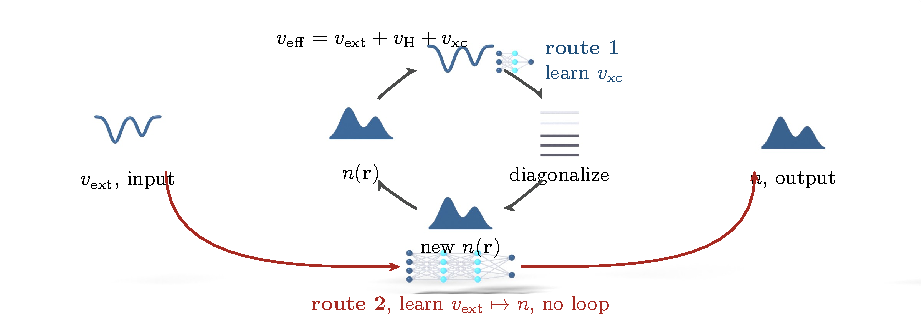
\includegraphics{figures/pdf/s10f04_dftml.pdf}
\end{aqmfigure}


This too is slides-and-transcript material with no notebook counterpart; DFT calculations were never
part of this course's numerical toolkit (\texttt{pyqula} is a tight-binding and mean-field library, not a
DFT code), so there is nothing to point you to beyond the derivation above.

\section{Phase classification: reusing the local-order-parameter-versus-topological-order split}

We come now to a section that is, in a real sense, a review of the whole course's classification
scheme, seen through a machine-learning lens. Throughout this course we have used two quite
different tools to tell phases apart. Sessions 1, 5, and 6 used a \textbf{local order parameter}: a
quantity built from a simple, local expectation value (charge imbalance for the CDW, magnetization
for the magnet, the pairing amplitude for the superconductor) that is zero in one phase and nonzero
in the other. Sessions 3 and 4 instead used a \textbf{topological invariant} (the Chern number, the Zak
phase) precisely because the phases in question are \emph{not} distinguished by any local quantity at
all; the distinction only becomes visible non-locally. Today's phase-classification example runs
exactly this contrast as an ``easy'' and a ``hard'' machine-learning worked example, and the lecture
itself frames it that way.

\textbf{The easy case: the Ising model.} Take classical Ising spins $\sigma_i = \pm 1$ on a square
lattice with the standard nearest-neighbor Hamiltonian and a local order parameter,

\begin{equation}
H_{\rm Ising} = -J\sum_{\langle i,j\rangle} \sigma_i \sigma_j, \qquad m = \frac{1}{N}\sum_i \sigma_i,
\end{equation}

which orders ferromagnetically ($|m|\to 1$) below a critical temperature $T_c$ and disorders
($m\to 0$) above it. Given only a single snapshot of the spin configuration, at some unknown
temperature, the phase is easy to read off even by eye: sum the spins and look at whether the
result is close to $\pm N$ or close to $0$. It is nonetheless a clean, controlled test case for
machine learning: train the very same cat-versus-dog architecture from Section 10.2 (input, the
$N\times N$ spin snapshot; output, a one-hot ordered/disordered label) on labeled snapshots below and
above $T_c$, and the classifier sharpens into a genuinely sharp transition as the system size grows
(the concrete sweep shown on the slides runs $L = 10$ up to $L = 60$), reproducing what we already
know analytically.

\textbf{The hard case: the Ising gauge theory.} Now replace the pairwise coupling with a \textbf{plaquette}
interaction, the product of the four spins around each elementary square of the lattice,

\begin{equation}
H_{\rm IGT} = -J\sum_{p} \prod_{i \in \partial p} \sigma_i,
\end{equation}

with the sum running over plaquettes $p$ and the product over the four spins sitting on the four
bonds that bound that plaquette; note that the spins here live on the \emph{links} of the lattice,
not on its sites. At zero temperature the ground state satisfies $\prod_{i\in\partial p}\sigma_i = +1$ on
\emph{every} plaquette, but this constraint is compatible with a macroscopic number of distinct spin
configurations (flipping the four spins on the bonds that meet at any single vertex, for instance,
leaves every plaquette product unchanged, since each of the four plaquettes touching that vertex
contains exactly two of those four bonds and every other plaquette contains none --- this local
gauge transformation is what gives the model its name). At infinite temperature, by contrast, plaquettes with product $+1$ and $-1$ occur with
equal probability. Crucially, both the ordered, constraint-satisfying configurations and the
disordered ones can look, individually, like a featureless $50/50$ mix of up and down spins: the
naive order parameter (10.9) that worked perfectly for the Ising model is \emph{useless} here, exactly
because this is a topological rather than a local-order transition, the same structural obstruction
that forced sessions 3 and 4 away from local order parameters and toward Chern numbers and Zak
phases. What (10.10) reproduces at the level of a toy classical model is the essential feature of
those earlier examples: the low-temperature and high-temperature phases are \textbf{topologically
distinct}, but nothing local tells them apart.

A convolutional neural network, trained on labeled low-$T$ and high-$T$ configurations with the same
supervised architecture as before, succeeds where the naive summary statistic fails; it is, in
effect, learning a nonlocal function of the spin configuration that plays the role a topological
invariant would play analytically. One further physical subtlety is worth stating precisely, since
it is easy to blur: the two phases here are separated by a \textbf{size-dependent crossover}, not a true
finite-temperature phase transition, so there is no sharp $T_c$ to converge to as the system grows,
unlike the genuine Ising transition of (10.9). What makes the machine-learning result genuinely
useful is that the trained network, having only ever seen one system size during training (the
slides show it trained at a single size and evaluated across $L = 4$ up to $L = 28$), correctly
captures this crossover across \emph{other} sizes and temperatures it was never trained on.
Figure~\ref{fig:s10:phaseclass} sets the easy and the hard case side by side in real space, which
is where the difference between them is actually visible.

% Session 10 -- phase classification: where a local order parameter works and where it fails.
% Placement: sec. "Phase classification", after the Ising-gauge-theory paragraph.
% Rendered by figures/blender/s10f05_phaseclassification.py, labels in figures/overlays/s10f05_phaseclassification.tex.
\begin{aqmfigure}{fig:s10:phaseclass}{Why one phase-classification problem is easy and the other is
hard, seen from above with $\sigma=+1$ raised and $\sigma=-1$ sunk. \textbf{(a,b)} For the Ising
model (10.9) the magnetization of a single snapshot already separates the phases, and a network
trained on such snapshots only finds again the logic of a local order parameter of sessions 1, 5 and
6. \textbf{(c,d)} For the Ising gauge theory (10.10) the spins live on the \emph{bonds}, and the
$T=0$ condition $\prod_{i\in\partial p}\sigma_i = +1$ leaves an exponentially large degenerate
manifold. A typical ground state is random from bond to bond, so the magnetization is $\approx 0$ in
both columns and no quantity on a single bond can distinguish them. The difference is in the
four-spin structure of the plaquettes, which is marked by a cross where the product is $-1$, and the
convolutional network has to find by itself a function of the configuration that is sensitive to it.
The shaded star in (c) is a gauge flip of the four bonds at one vertex, which keeps every plaquette
product. This is the same obstruction that forced sessions 3 and 4 to go from local order parameters
to Chern numbers and Zak phases.}
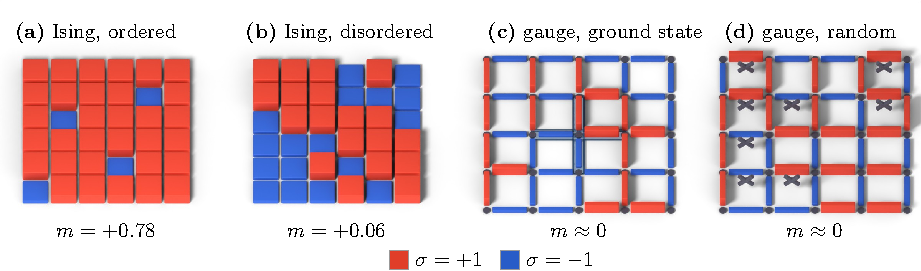
\includegraphics{figures/pdf/s10f05_phaseclassification.pdf}
\end{aqmfigure}


\section{Hamiltonian learning: the inverse of session 1's opening move}

We come, finally, to the piece of today's material that closes the loop most explicitly. Go back to
session 1, Section 1.4: every quantum mechanical system is governed by the Schr\"odinger equation,
and given a Hamiltonian (and an initial state) we can integrate forward and obtain, in principle,
every observable the system will ever show us: density, magnetization, response functions, and so
on. That forward arrow, Hamiltonian $\to$ observable, is what essentially this entire course has
been built to compute, one physical setting at a time.

But it is not the arrow an experimentalist actually gets to use. A real measurement never hands you
the Hamiltonian; it hands you an observable directly, a density, a conductivity, an ARPES spectrum,
a neutron-scattering structure factor, and the Hamiltonian is exactly the thing you do \emph{not} have
and would like to infer. \textbf{Hamiltonian learning} poses this explicitly as the inverse problem: the slides write the
Hamiltonian itself as $H(\lambda_i, w_i)$, splitting its dependence into the physical parameters of
interest $\lambda$ (magnetic or electric fields, hopping amplitudes, many-body interaction
strengths) and a set of ``hidden,'' or nuisance, variables $w$ one does \emph{not} want to fit (smaller
marginal parameters, disorder realizations, artifacts of whichever computational method generated
the training data, plain randomness). Writing $\mu \equiv w$ for that hidden-variable vector, the
forward direction is the map

\begin{equation}
\mathcal{O} = \mathcal{O}\big[H(\lambda,\mu)\big],
\end{equation}

and Hamiltonian learning asks for the inverse map, $\mathcal{O} \mapsto \lambda$, marginalizing over
$\mu$ as best we can rather than trying to fit it. This is a genuinely difficult inverse problem in
general (many different $\lambda$ can be compatible with the same measured $\mathcal{O}$, and real
experimental data to train on is scarce), and the practical strategy is, once again, to lean on
theory to make up for the shortage of experiment. Simulate the observable $\mathcal{O}$ from many
different, \emph{known} Hamiltonians $H(\lambda_n)$ spanning the parameter range of physical interest
(the same forward calculations, density, magnetization, spectroscopy, that earlier sessions taught
us to compute directly), and train a neural network $\mathcal{N}_\theta$ on this synthetic data to
invert (10.11), minimizing

\begin{equation}
\mathcal{L}(\theta) = \sum_n \left\| \mathcal{N}_\theta\big(\mathcal{O}[H(\lambda_n)]\big) - \lambda_n \right\|^2.
\end{equation}

Once trained on simulated pairs where the answer $\lambda_n$ is known by construction, the same
network is applied to a genuine experimental observable $\mathcal{O}_{\rm exp}$ (a two-dimensional
spectroscopy of a quantum magnet is the concrete example the lecture used), and $\hat\lambda =
\mathcal{N}_\theta(\mathcal{O}_{\rm exp})$ gives an estimate of the physical Hamiltonian parameters,
for instance the first-, second-, and third-neighbor exchange couplings of that magnet, extracted
directly from a measurement with no closed-form inversion formula available at all.
Figure~\ref{fig:s10:hamlearning} lays out both stages, the synthetic training set and the
deployment on real data, against the forward arrow they are jointly inverting.

% Session 10 -- Hamiltonian learning: the forward arrow of the whole course, its inverse, and
% Placement: sec. "Hamiltonian learning", after equation (10.12).
% Rendered by figures/blender/s10f06_hamiltonianlearning.py, labels in figures/overlays/s10f06_hamiltonianlearning.tex.
\begin{aqmfigure}{fig:s10:hamlearning}{Hamiltonian learning, and why it closes the loop of the
course instead of going outside it. \textbf{Top.} The forward arrow $H\mapsto\mathcal{O}$ of (10.11)
is what sessions 1 to 9 built during all their time. The arrow that an experiment needs goes in the
other direction, and there is no closed-form inversion of it. \textbf{(a)} The solution to the lack
of experimental training data is to produce the data. We simulate $\mathcal{O}$ from many
\emph{known} Hamiltonians, so that every training pair comes with its answer $\lambda_n$ by
construction, and we fit the network with (10.12). \textbf{(b)} Only after this step the trained
network is applied to a real measurement. Note what the training set is made of, which is the
forward methods of the whole course, run many times. The final method of the course and its first
method are the same method, applied in opposite directions.}
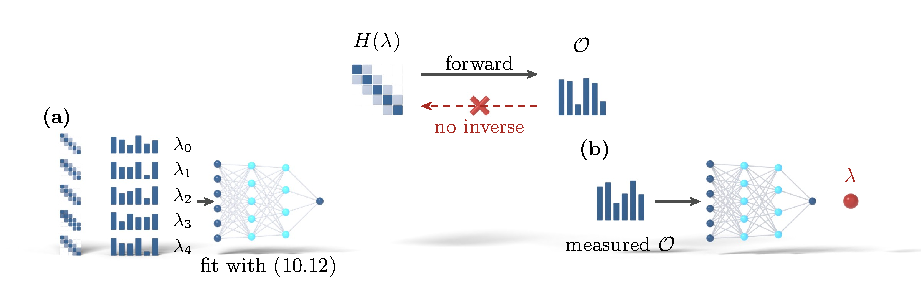
\includegraphics{figures/pdf/s10f06_hamiltonianlearning.pdf}
\end{aqmfigure}


This is the literal mirror image of session 1's opening framing, and it is worth sitting with that
symmetry for a moment. We spent nine sessions building increasingly sophisticated ways to go from a
Hamiltonian to an observable: mean-field decoupling, Bloch's theorem, topological invariants, Landau
levels, Nambu spinors, magnon spectra, tensor-network ground states, parton constructions, and
response functions. Hamiltonian learning does not abandon any of that; it uses exactly that forward
machinery, run many times over on synthetic data, as the training set for learning to run the
process in reverse. The course's method and the course's final method are, in that sense, the same
method, pointed in opposite directions.

\section{Closing summary}

\begin{itemize}
\item A deep neural network is a parametric function trained by minimizing a loss function via gradient
  descent, equation (10.1); every other construction in this session is a specific choice of input,
  output, and loss built on top of that one template.
\item \textbf{Neural network quantum states} replace explicit storage of a wavefunction's $2^L$ coefficients
  with a network $C_\theta(s)$, equation (10.2), trained by treating the variational energy itself as
  the loss function, equations (10.3)-(10.5); NNQS sits above matrix product states and PEPS in the
  variational hierarchy, imposing the least structure of any ansatz this course has used. The same
  ansatz, fitted by maximum likelihood instead of energy minimization, solves quantum state
  tomography with far fewer than $2^L$ measurements.
\item \textbf{Tensor networks}, built from the matrix product state ansatz (10.6) and its tree/MERA/PEPS
  generalizations, can be run in reverse as machine-learning architectures; applied to image
  classification (Fashion-MNIST), this reaches 95.38\% training and 88.97\% test accuracy, competitive
  with conventional neural networks.
\item \textbf{Density functional theory} rests on the Hohenberg-Kohn functional (10.7) and the Kohn-Sham
  self-consistency loop (10.8); machine learning enters either by learning the unknown
  exchange-correlation piece of (10.8) (self-consistency loop unchanged) or by learning the entire
  potential-to-density map directly (self-consistency loop removed entirely).
\item \textbf{Phase classification} reuses this course's local-order-parameter-versus-topological-order split
  one more time: the Ising model (10.9) is the easy, locally-detectable case (sessions 1/5/6's
  logic), while the Ising gauge theory (10.10) is the hard, topologically-distinct-phases-with-no-
  local-order-parameter case (sessions 3/4's logic), and a trained network succeeds where the naive
  order parameter fails.
\item \textbf{Hamiltonian learning} poses the inference of a Hamiltonian from measured observables,
  equation (10.11), as the literal inverse of session 1's opening move; training a network on
  synthetic forward data, equation (10.12), and applying it to real experimental observables lets us
  close that loop in practice, not just in principle.
\end{itemize}

We opened this course by asking how a handful of identical atoms, arranged into a lattice, could
produce a phenomenology as rich as the one we spent ten sessions touring: charge density waves,
magnets, superconductors, topological insulators, fractional excitations, spin liquids, and more,
none of it visible in a single atom on its own. Answering that question took us through second
quantization and mean-field theory, through Bloch's theorem and topological invariants, through
Nambu spinors and magnon spectra, through tensor networks and parton constructions, and through
linear response as a diagnostic across all of it. Today's session closed that arc twice over: once
by showing that a neural network can stand in for the many-body wavefunction itself, and once by
showing that the entire forward machinery of the course, Hamiltonian in, observable out, can be run
backward to infer the Hamiltonians that real materials actually have. That is a fitting place to
leave things: not with a final answer, but with a general-purpose way of asking the question again,
for whichever quantum material comes next.
